% !TEX root = ../main.tex
\documentclass[../main.tex]{subfiles}


\begin{document}
\section{User authentication and authorization}

\subsection{Backed integration}

\subsubsection{Structure}

The code responsible for handling user authorization is located
under \texttt{src/auth} directory in the \textbf{backend} app directory.

\begin{figure}[H]
  \centering
  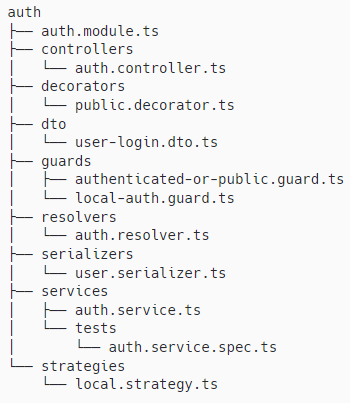
\includegraphics{file-tree/backend-auth-tree.png}
  \caption{Backend auth directory structure}
\end{figure}

The \texttt{auth} directory is further divided into following sub-directories:
\begin{itemize}
  \item \texttt{controllers} - contains code which is responsible for handling incoming HTTP requests and sending back responses (REST API)
  \item \texttt{decorators} - contains code that is used to extend other functions with additional functionality
  \item \texttt{dto} - contains data transfer objects, which define the data that is exchanged using REST API
  \item \texttt{guards} - contains code that is used to determinate if a given request should be authorized or not
  \item \texttt{resolvers} - contains GraphQL resolvers, which are used to handle incoming GraphQL requests
  \item \texttt{serializer} - contains code that is used to covert object to a representation that can be stored in cache
  \item \texttt{services} - contains classes that defined the business logic of the enclosing module, in this case the business logic is related to user authentication and authorization
\end{itemize}
This file structure is also used in other module of the backend application. It is a common practice to divide code into such sub directories in NestJS applications.
To emphasize the role which each file plays an additional suffix is added to the file name. For example, \texttt{auth.controller.ts} is a controller file, \texttt{auth.service.ts} is a service file, etc.

In NestJS the application is build with modules, each module resides in its own directory under the \texttt{src} directory.
Modules have to defined what service is exposed to other modules and what is imported from other modules. In a special module class
which is often stored in a file suffixed with \texttt{.module.ts}. In this case the module class is defined in \texttt{auth.module.ts} file.

\begin{listing}[H]
  \tsfile{implementation/code/auth/auth.module.ts}
  \caption{Auth module class}
  \label{lst:auth-module}
\end{listing}

The module class is created using the \texttt{@Module} decorator imported from NestJS library.
The purpose of fileds of the module class decorator are as follows:
\begin{itemize}
  \item \textbf{imports} - defines what other modules are imported into the current module
  \item \textbf{providers} - contain list of services, resolvers and guards that are provided by the current module for the application
  \item \textbf{controllers} - defines what controllers are provided by the current module
  \item \textbf{exports} - defines what services, resolvers and guards are exported from the current module and can be used by other modules
\end{itemize}

\subsubsection{Passport.js integration}

Passport.js is a library that handles the authentication logic in the application.
To integrate passport into the application first a strategy has to be defined. In this case the \texttt{LocalStrategy} is used.
This strategy performs using the username and password provided by the user. The logic of the strategy is defined in \texttt{local.strategy.ts} file.

\begin{listing}[H]
  \tsfile{implementation/code/auth/local.strategy.ts}
  \caption{Local strategy implementation}
\end{listing}

In this application the \textbf{email} field will be used as the username. For Passport to be able to properly parse the login DTO the
\texttt{usernameField} property has to be set to \texttt{email}. The \texttt{validate} method is used to validate the user credentials.

The defined strategy is then used to define an \texttt{AuthGuard} which will perform the authentication logic and reject the request if the user
did not pass the authentication credentials (username and password for the \texttt{LocalStrategy}).

\begin{listing}[H]
  \tsfile{implementation/code/auth/local.strategy.ts}
  \caption{Local strategy guard}
\end{listing}

This guard is then used to decorate a controller method.

\begin{listing}[H]
  \tsfile{implementation/code/auth/local-guard-usage.ts}
  \caption{Local strategy guard usage example}
  \label{code:local-guard-usage}
\end{listing}

Posting a request to the \texttt{/login} endpoint will first invoke the \texttt{LocalAuthGuard}.
This guard will inspect the request object for user credentials and if they are not present it will reject the request.
If the credentials are present the \texttt{validate} method of \texttt{LocalAuthGuard} will be invoked and the validation succeeds then request will be authorized, and the
\texttt{login} method will be invoked. Otherwise, the request will be rejected and the \texttt{UnauthorizedException} will be thrown.

To complete the authentication the result of the \texttt{login} method has to be serialized and stored in the session.
To later de-serialize the session middleware has to be registered in the application.

\begin{listing}[H]
  \tsfile{implementation/code/auth/express-session.middleware.ts}
  \caption{Express session middleware}
\end{listing}

The express middleware will write and retrive the session data from the Redis cache and store it in the \texttt{req.session} object.
A session cookie will be sent to the client and the client will send it back with each request. The session cookie will be used to identify the session.
The data that is stored in the session is provided by the passport middleware.

\begin{figure}[H]
  \centering
  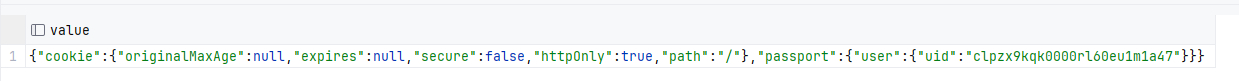
\includegraphics[width=\textwidth]{auth/redis-data.png}
  \caption{Session data stored in Redis}
\end{figure}


\begin{listing}[H]
  \tsfile{implementation/code/auth/passport.middleware.ts}
  \caption{Passport session middleware}
\end{listing}

\subsubsection{Route authentication}

The \texttt{LocalAuthGuard} is used to authenticate the user when they are logging in. To authenticate the user when they are accessing a protected route
a separate guard has to be defined. The guard will read the session data from the request object and check if the user is authenticated.
This logic is defined in \texttt{AuthenticatedOrPublic} guard, which is employed throughout the entire application to guarantee that only authenticated users have access.


To allow access to certain routes for unauthenticated users, a decorator named \texttt{PublicHandler} was introduced. This decorator is utilized to annotate controllers and resolvers.

\begin{listing}[H]
  \tsfile{implementation/code/auth/public.decorator.ts}
  \caption{Public decorator implementation}
\end{listing}

To implement this decorator the special object called \texttt{Reflector} is used. This object is provided by the NestJS framework and is used to read and write metadata.
This is similar to annotations in \texttt{Java} or \texttt{C\#} languages. The metadata can be written to a class, method or a property. In this case the metadata is written to a class, that uses the \texttt{PublicHandler} decorator.
Later this metadata is read by the \texttt{AuthenticatedOrPublic} guard to determine if the route should be accessible by unauthorized users.

\begin{listing}[H]
  \tsfile{implementation/code/auth/authenticated-or-public.guard.ts}
  \caption{Authenticated or public guard implementation}
\end{listing}

The login router is an example of a route that is accessible by unauthenticated users. The \texttt{PublicHandler} decorator is used to mark the \texttt{login} method as public.

\begin{listing}[H]
  \tsfile{implementation/code/auth/login-full.controller.ts}
  \caption{Full login router implementation}
\end{listing}

\subsubsection{Permission system}

The permissions system implementation is located in the \texttt{src/rbac} directory. The directory structure is similar to the \texttt{auth} directory structure.

\begin{figure}[H]
  \centering
  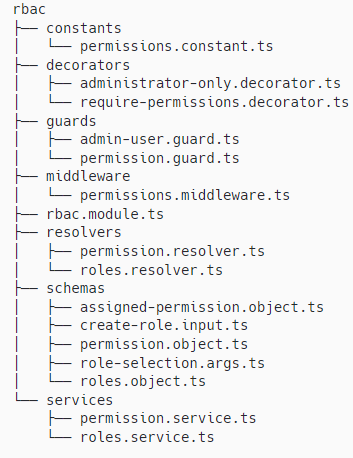
\includegraphics{file-tree/backend-rbac-tree.png}
  \caption{Backend rbac directory structure}
\end{figure}

Permissions are defined in the \texttt{permissions.constant.ts} file. These permissions are inserted into the database during the database seeding process.
\begin{figure}[H]
  \centering
  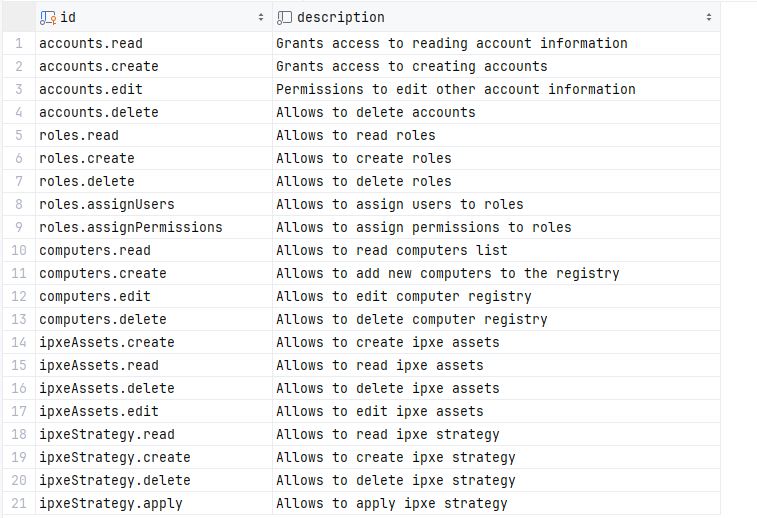
\includegraphics[width=\textwidth]{auth/db-permissions.png}
  \caption{Permissions stored in the database after seeding}
\end{figure}

Each permission is defined by a unique identifier and a description. The identifier consist of category for which functionality the permission is defined and the name of the individual permission.
The permissions system provides two decorators:
\begin{itemize}
  \item \textbf{RequirePermission} - Takes a list of permissions as an argument and assigns the metadata to the decorated class, method or property
  \item \textbf{AdministratorOnly} - Assigns metadata information that the decorated class, method or property can only be accessed by users with the \texttt{ADMIN} account type
\end{itemize}

Permission system also define a middleware which checks the user permissions and assign them to the request object.

\begin{listing}[H]
  \tsfile{implementation/code/auth/permission.middleware.ts}
  \caption{Permissions middleware implementation}
\end{listing}

This module defines two global guards which read the metadata set from permission decorators and check if the user has the required permissions to access the route.
If user does not have the required permissions the request is rejected with HTTP status code \texttt{403 Forbidden}.

\subsubsection{Roles creation and assignment}

The role retrieval and creation is implemented in the \texttt{RoleResolver} class. This class handles GraphQL queries and mutations related to roles.
The exchanged data format is defined under the \texttt{schemas} sub directory. Under this directory there types of files can be found:

\begin{itemize}
  \item \textbf{.object.ts} - Object types, used to define the shape of the data that is exchanged between the client and the server through GraphQL API
  \item \textbf{.input.ts} - Input types, used to define the shape of the data that is sent to the server
  \item \textbf{.args.ts} - Similar to input types, but instead of defining the shape in object notation, the shape defined duration function arguments
\end{itemize}

\begin{listing}[H]
  \tsfile{implementation/code/auth/role.object.ts}
  \caption{Role object returned from the server}
\end{listing}

Object types in GraphQL APIs often contain another object types. In this case the \texttt{Role} object contains a list of \texttt{Permission} objects.
In contrast to the REST API design where only the relation keys would be returned for permissions, GraphQL APIs are designed in this way to reduce the number of requests that have to be made to the server.
This hover poses an implementation challenge as the full data object alongside with all of its nested objects have to be returned from the database.
GraphQL provides a solution to this problem in the form of \texttt{FieldResolvers} which are used to resolve nested objects.

\begin{listing}[H]
  \tsfile{implementation/code/auth/role.resolver.ts}
  \caption{Fragemnt of the role resolver implementation}
\end{listing}

The above listing shows a fragment of the implementation of the \texttt{roles} resolver.
The mutations are marked with the \texttt{@Mutation} decorator and the arguments are defined using the \texttt{@Args} decorator.
Both \texttt[ArgTypes] and \texttt{InputTypes} can be used to define the shape of the arguments.
Field resolvers take single argument which is the object that is being resolved. In this case the \texttt{Role} object is being resolved.
They are responsible for resolving the nested field after which the method is named.

Resolvers heavily rely on the services to perform the business logic. In this case this logic is defined in the \texttt{RolesService} class.
Services are injected though the constructor function which in the case of listing \ref{code:auth-resolver} was omitted for brevity.


\subsubsection{Admin login as other user}

The last functionality that is implemented by the authorization and authentication system is the ability for the administrator to login as another user.
This functionality is implemented in the \texttt{AuthResolver} class. This resolver is used to handle GraphQL requests related to authentication and authorization.

\begin{listing}[H]
  \tsfile{implementation/code/auth/auth.resolver.ts}
  \caption{Auth resolver implementation}
  \label{code:auth-resolver}
\end{listing}

This resolver handles the \texttt{adminLoginAsUser} mutation. Frontend application can use this mutation to login as another user.
Resolver uses the \texttt{AdministratorOnly} decorator to ensure that only users with the \texttt{ADMIN} account type can use this mutation.
This mutation takes one parameter which is the unique identifier of the user that the administrator wants to log in as.

\begin{listing}[H]
  \graphqlfile{implementation/code/auth/login-as-mutation.gql}
  \caption{Login as another user graphql mutation}
  \label{code:login-as-mutation}
\end{listing}

\subsection{Frontend integration}

\subsubsection{Login page}

The default route of the frontend application for unauthenticated users is the login page. This page is implemented in the \texttt{LoginPage} component
located in directory \texttt{src/app/login/page.tsx}. Next.js read the contents of this file and provides it to user when they navigate to \texttt(/login) route.

\begin{listing}[H]
  \jsxfile{implementation/code/auth/login-page.tsx}
  \caption{Login page component implementation. This is a server component}
\end{listing}

Login form is showed to the user if they are not authenticated.
If authenticated user tries to access the login page they will be redirected to the home page.

\begin{figure}[H]
  \centering
  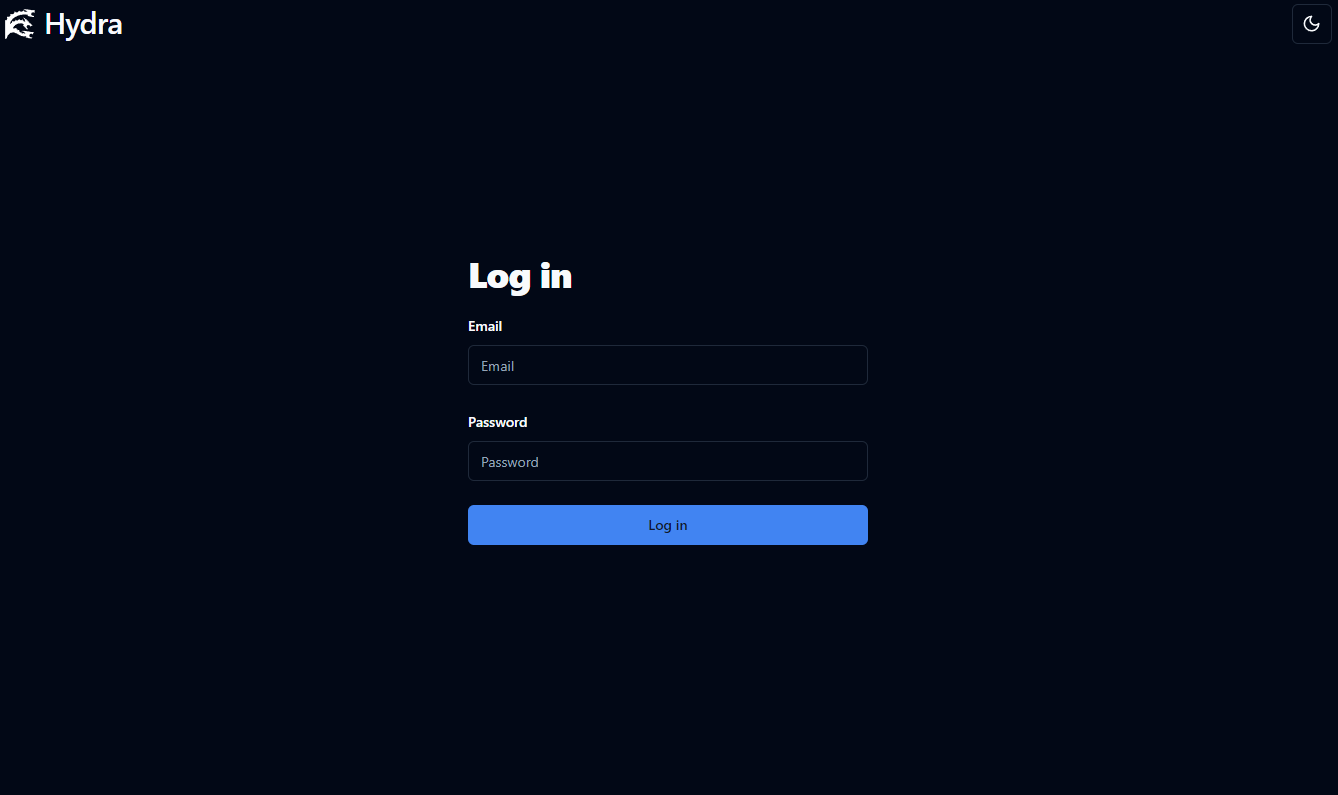
\includegraphics[width=\textwidth]{auth/screens/login.png}
  \caption{Login page}
\end{figure}

The automatic redirection of unauthorized users is implemented in the Next.js application middleware located in \texttt{src/middleware.ts} file.

\begin{listing}[H]
  \tsfile{implementation/code/auth/next-middleware.ts}
  \caption{Next.js middleware for redirecting unauthorized users}
\end{listing}

\subsubsection{Roles page}

The root server component for the roles page fetches the data form server GraphQL API and passes it to the \texttt{DataTable} component.
DataTable is a table with advanced filtering and sorting capabilities. It is implemented using the \texttt{TanStack Table} library \cite{tanstack-table}.

\begin{listing}[H]
  \jsxfile{implementation/code/auth/roles-page.tsx}
  \caption{Roles page component implementation. A fallback component is shown if the user last sufficient permissions}
\end{listing}

\begin{figure}[H]
  \centering
  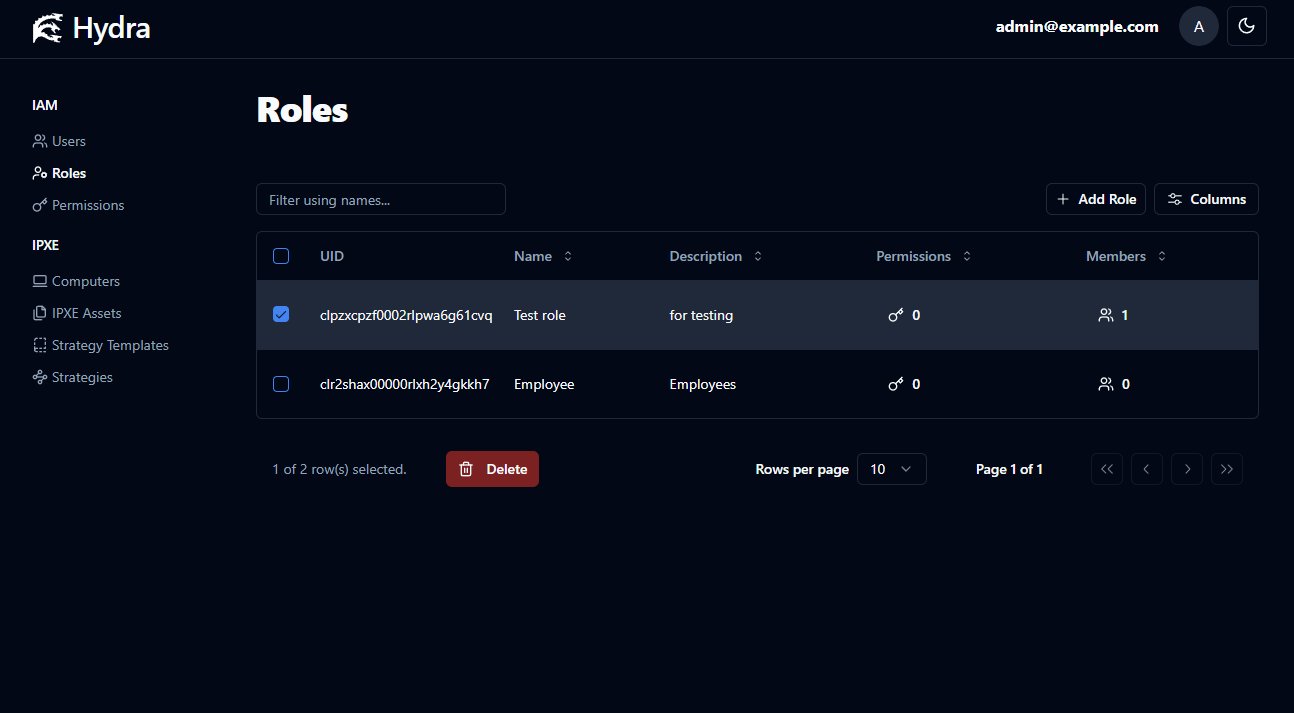
\includegraphics[width=\textwidth]{auth/screens/roles.png}
  \caption{Roles page}
\end{figure}

Data table supports disabling selected columns, searching and sorting. It also supports pagination.
After selecting a row a delete button is shown. This button is disabled if the user does not have sufficient permissions.

\begin{figure}[H]
  \centering
  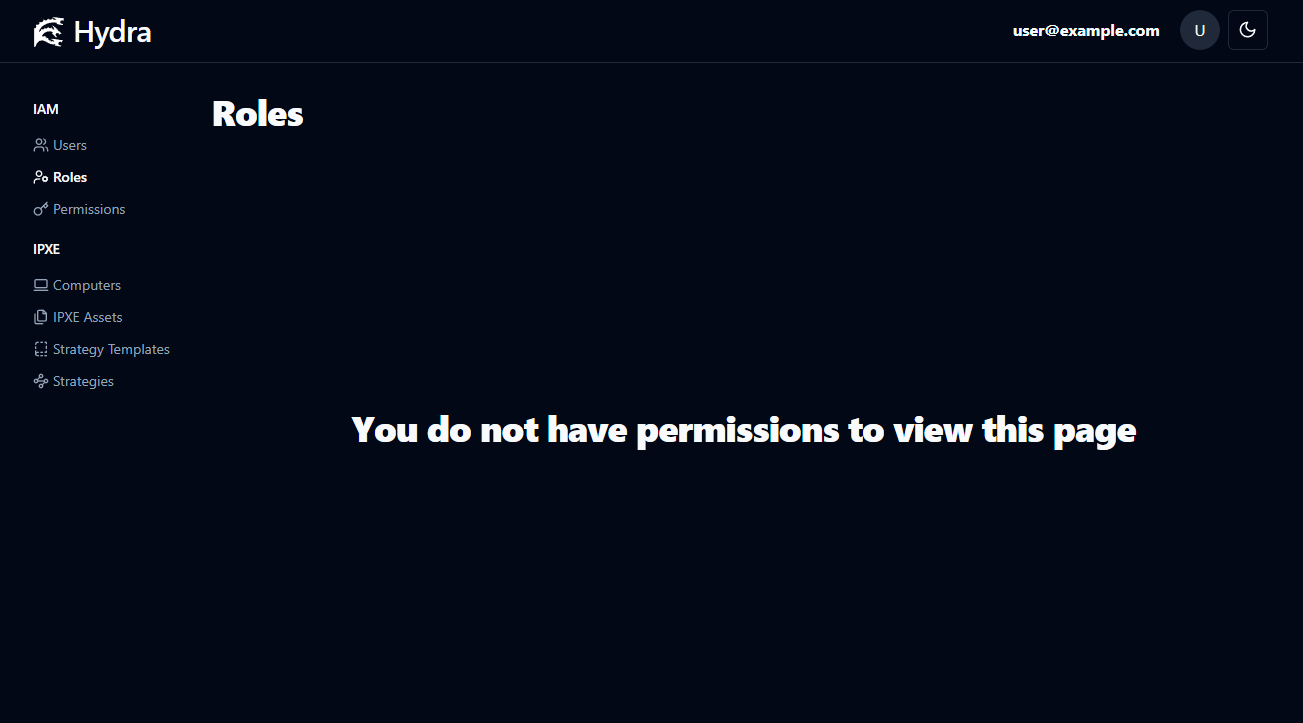
\includegraphics[width=\textwidth]{auth/screens/roles-fallback-page.png}
  \caption{Roles page fallback component}
\end{figure}

Permissions columns show the number of assigned permission to a given role.
Similarly the members column shown number of users that have been assigned a given role.
Clicking on these number will open a model with transfer list component which can be used to assign permissions or users to a given role.

\begin{figure}[H]
  \centering
  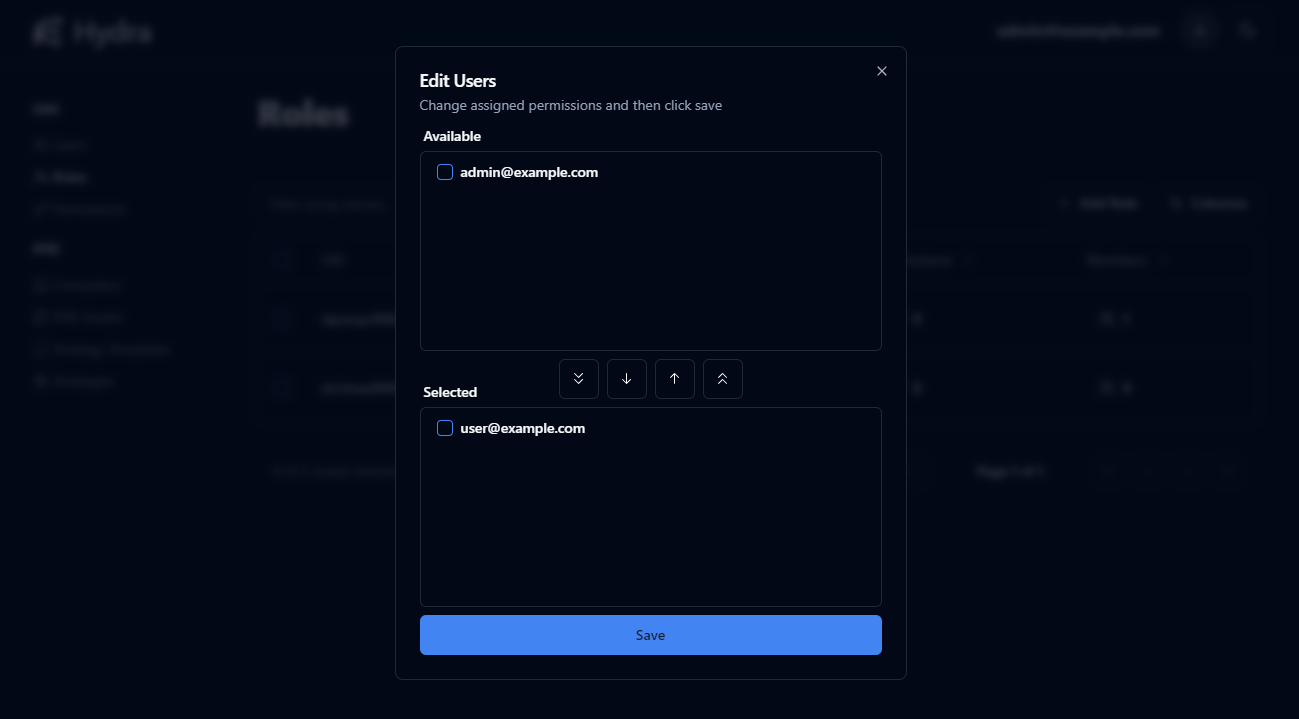
\includegraphics[width=\textwidth]{auth/screens/editing-user-roles.png}
  \caption{Assigning role to users}
\end{figure}

Each data mutation like creating, updating or deleting a role is performed though the use of GraphQL mutations.
Additionally a toast notification is shown to the user to inform them about the result of the operation.

\begin{figure}[H]
  \centering
  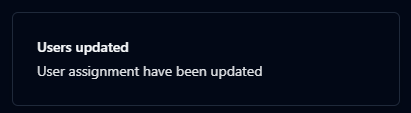
\includegraphics{auth/screens/toast-example.png}
  \caption{Example toast notification information the user about the result of the operation}
\end{figure}

To add new role the user has to click on the \texttt{Add role} button. This will open a modal with a form that can be used to create a new role.

\begin{figure}[H]
  \centering
  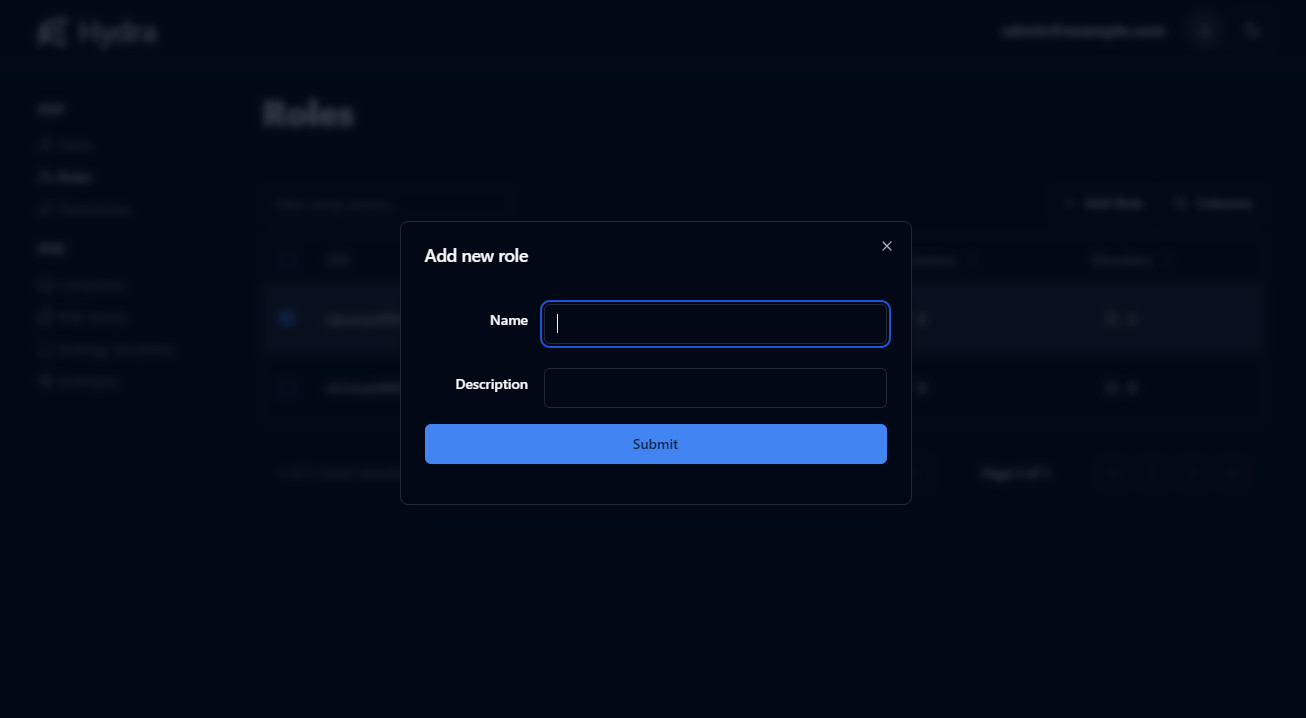
\includegraphics[width=\textwidth]{auth/screens/add-role.png}
  \caption{Add role modal}
\end{figure}

\subsubsection{Permission page}

Permissions page serve the singular purpose of showing the user what permissions are available in the system.
As this view is not used to perform any data mutations it is implemented using regular table component rather than the data table component.

\begin{figure}[H]
  \centering
  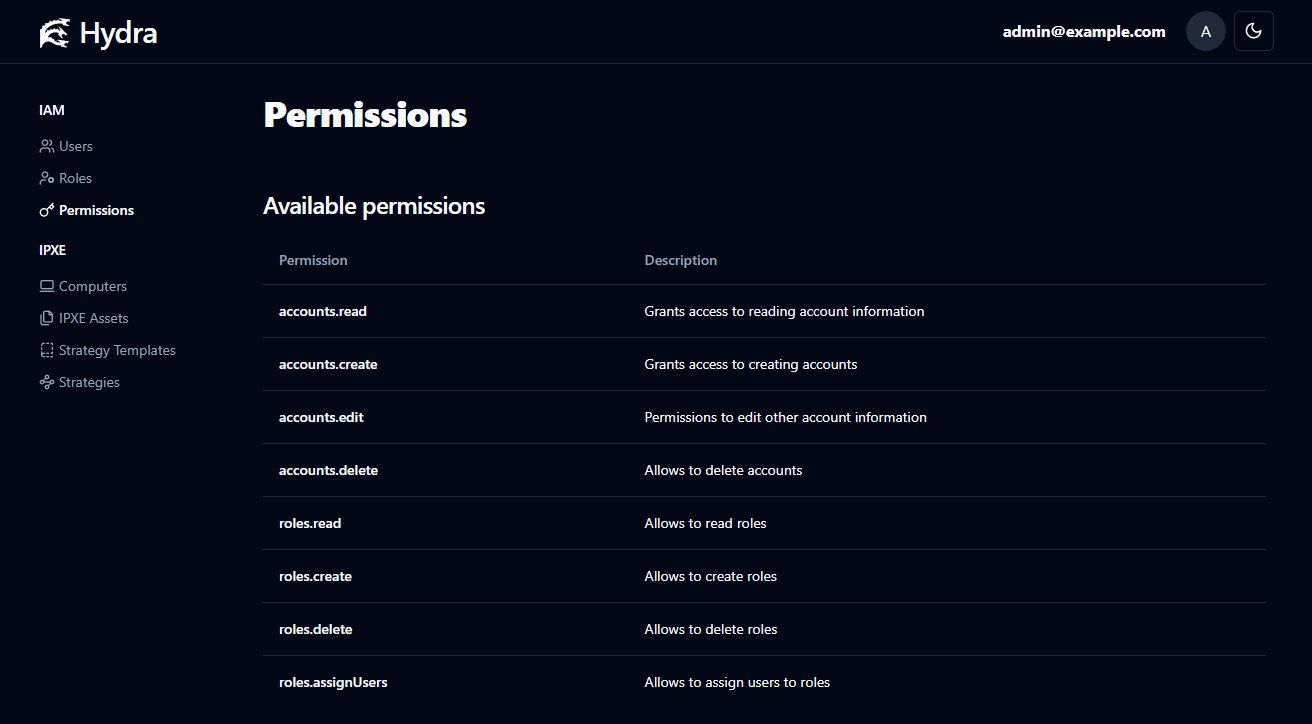
\includegraphics[width=\textwidth]{auth/screens/permissions.png}
  \caption{Permissions page}
\end{figure}

\subsubsection{Users page}

The last page that is implemented as a part of the authorization and authentication system is the users page.
This page is implemented in the \texttt{UsersPage} component located in the \texttt{src/app/dashboard/users/page.tsx} file.
This view allow for viewing, creating, updating and deleting users.
Its design is similar to the design of the roles page. It uses the same data table component to display the data.

\begin{figure}[H]
  \centering
  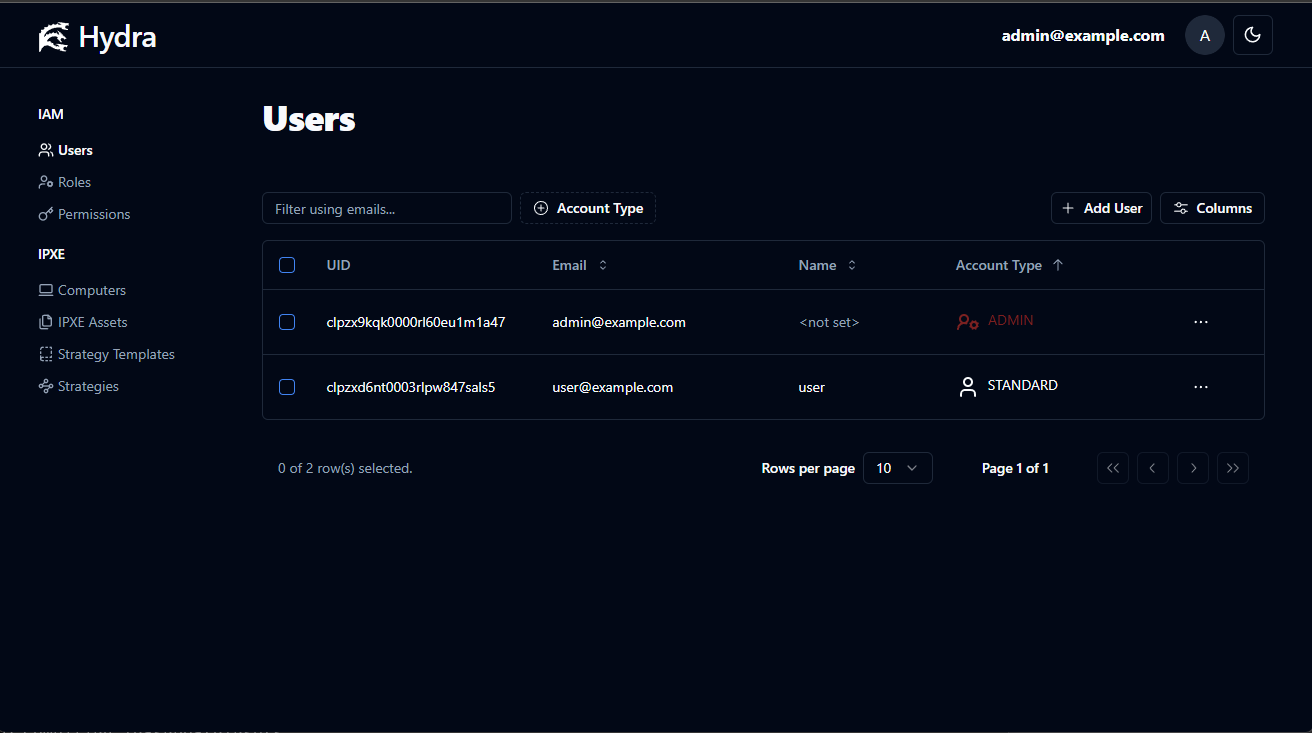
\includegraphics[width=\textwidth]{auth/screens/users.png}
  \caption{Users page}
\end{figure}

This views data table feature row context menu which can be used to perform actions on a given user.
The presented actions depend on logged-in user permissions.

\begin{figure}[H]
  \centering
  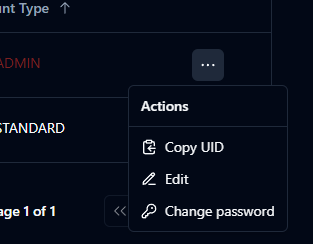
\includegraphics{auth/screens/user-actions.png}
  \caption{User context menu}
\end{figure}

\end{document}